% This is LLNCS.DEM the demonstration file of
% the LaTeX macro package from Springer-Verlag
% for Lecture Notes in Computer Science,
% version 2.4 for LaTeX2e as of 16. April 2010
%
\documentclass{llncs}
%
%\usepackage{makeidx}  % allows for indexgeneration
\usepackage{wrapfig}
\usepackage{float}
\usepackage[english]{babel}
\usepackage{lipsum}
\usepackage{caption}
\usepackage{subcaption}
\usepackage{graphicx}
	\graphicspath{{images/}} 
%\usepackage{cite}
\usepackage[linesnumbered,ruled]{algorithm2e}
\usepackage{courier}
\usepackage{hyperref}
    \hypersetup{colorlinks=true,allcolors=blue}
\usepackage{listings}
	\lstset{
  		basicstyle=\ttfamily,
  		frame=none, 
  		breaklines=true,
  		numbers=left,
  		xleftmargin=2.5em,
  		framexleftmargin=0em,
    	emphstyle=\textbf,
    	float=t
	}
	\lstdefinestyle{ocl}{
  		emph={
        	context, inv
    	}
	}
	\lstdefinestyle{cbp}{
	    basicstyle=\ttfamily\scriptsize,
  		emph={
        	session, create, of, type,
        	set, to, add, hire
    	}
	}
	\lstdefinestyle{xmi}{
		basicstyle=\ttfamily\scriptsize,
  		emph={
        	Node, children
    	}
	}
	\lstdefinestyle{xml}{
	    basicstyle=\ttfamily\scriptsize,
  		emph={
        	register, create, add, to, resource,
        	from, eattribute, remove, ereference,
        	set, unset, session, Roy, Jen,
        	Moss, Richmond
    	}
	}
	\lstdefinestyle{java}{
	    basicstyle=\ttfamily\scriptsize,
  		emph={
        	case, UNSET,
        	instanceof, else, if, void,
        	new, UnsetEAttributeEvent,
        	UnsetEReferenceEvent,
        	@override, public, class, extends
    	}
	}
	\lstdefinestyle{eol}{
	    basicstyle=\ttfamily\scriptsize,
  		emph={
        	var, new, for, in, create, set, of, with, 
        	unset, to, add, remove, delete, register,
        	from, position, from, move-within, session, \.
    	}
	}

\begin{document}
\renewcommand{\thelstlisting}{\arabic{lstlisting}}
\renewcommand{\labelitemi}{$\bullet$}
\newcommand{\dk}[1]{\textbf{[DK: #1]}}

\title{An Algorithm for Efficient Loading \\ of Change-Based Models}
%
%\titlerunning{Change-based Persistence and Its Loading Optimisation}  % abbreviated title (for running head)
%                                     also used for the TOC unless
%                                     \toctitle is used
%
\author{
    Anonym%Alfa Yohannis \and Dimitris Kolovos \and Fiona Polack 
}
%
\authorrunning{
    Anonym%Alfa Yohannis et al.
} % abbreviated author list (for running head)
%
%%%% list of authors for the TOC (use if author list has to be modified)
%\tocauthor{Dimitris Kolovos, Fiona Polack, Alfa Yohannis}
%

\institute{anonym}
%\institute{Department of Computer Science, University of York, United Kingdom\\
%\email{\{ary506, dimitris.kolovos, fiona.polack\}@york.ac.uk}}

\maketitle              % typeset the title of the contribution

\begin{abstract}
We propose a change-based approach for persisting models that conform to object-oriented (MOF/Ecore) metamodelling architectures. We demonstrate how change-based persistence can preserve fine-grained changes to models and facilitate high-performance incremental model processing (e.g. transformation, validation) through fast model change detection. We illustrate a language-independent change-based model representation format, and an optimised model loading algorithm that seeks to avoid replaying changes that have no impact on the eventual state of the model. We report on benchmarks that compare model loading and saving performance of the proposed change-based representation against the standard state-based representation format (XMI). Our results show considerable savings in terms of persisting and identifying changes made to models at an increased---but linear---model loading cost.
\end{abstract}

\section{Introduction}
\label{sec:introduction}
Existing approaches for file-based persistence of models in metamodelling architectures such as MOF and EMF are predominately state-based. In such approaches, model files contain snapshots of the models' contents and activities such as version control and change detection are left to external systems such as file-based version-control systems and model differencing facilities. Activities such as model comparison and change detection are computationally consuming for state-based models and can become a burden as larger models are developed in a collaborative setting, but also for incremental model processing \cite{rath2012derived}, \cite{ogunyomi2015property}. 

In contrast to persisting \textit{snapshots} of models, we are exploring a change-based approach that persists \textit{changes} made to models instead. The change-based approach comes with a number of envisioned benefits over stated-based persistence, such as the ability to detect changes much faster and more precisely, which can then have positive knock-on effects on helping developers to diff/merge models in collaborative modelling environments, as well as supporting faster incremental model validation and transformation. Change-based persistence comes with a downside---an increased load cost---since all recorded changes need to be replayed to reconstruct a model's state.   

Our work extends the previous work of Yohannis et al. \cite{yohannis2017turning} that implements a change-based persistence (CBP) format, which has not addressed the load cost, by proposing and evaluating an algorithm that reduces loading time of change-based models by avoiding replaying changes that have no impact on the eventual state of the model (e.g. that are cancelled out by subsequent changes). We assess the efficiency of the algorithm in terms of persistence and loading time, and memory footprint. Our approach demonstrates considerable savings in time for persisting and identifying changes made to models, at a higher, but linear, model loading cost, compared to state-based models when tested on large scale models. %\dk{If the contribution we're proposing in this paper is the optimised loading algorithm, starting that loading cost is higher can be confusing.}

The rest of the paper is structured as follows. Section \ref{sec:case_study} introduces two running examples and provides a brief overview of the change-based model persistence we extend. Section \ref{sec:loading_time_optimisation} presents an algorithm that intends to speed up loading of change-based models, and its supporting data structures %\dk{Merge Sections 3 and 4}.  
Sect. \ref{sec:performance_evaluation} shows the results of controlled evaluation experiments for assessing the benefits of the proposed algorithm. Section \ref{sec:related_work} provides an overview of existing related work. Section \ref{sec:limitations} discusses the limitations of our approach and Sect. \ref{sec:conclusions} concludes this paper.

\section{Running Example}
\label{sec:case_study}
To help us explain the optimisation algorithm, we use tree model. We choose it because we want to start with a simple example to help readers understand our approach and it has a reasonable coverage of EMF framework's features such as single/multi valued, containment/non-containment, and attribute/reference, and the tree nature of the Eclipse Modelling Framework (EMF) models (e.g. XMI format). Figure \ref{fig:node_metamodel} show the three model's metamodel. The model consists of nodes in which every node can have one or many, containment references to other nodes (\emph{children} relationship). A node also has a have a single non-containment reference to another node (\emph{parent} relationship). Every node has a string attribute \emph{name} and a multi-valued, integer attribute \emph{values}. 

\begin{figure}[ht]	
	\begin{subfigure}[t]{0.5\linewidth}
		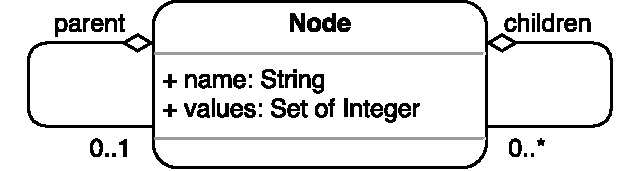
\includegraphics[width=0.9\linewidth]{node_metamodel}
    \caption{The tree metamodel.}
    \label{fig:node_metamodel}
	\end{subfigure}
	\hfill
	\begin{subfigure}[t]{0.5\linewidth}
		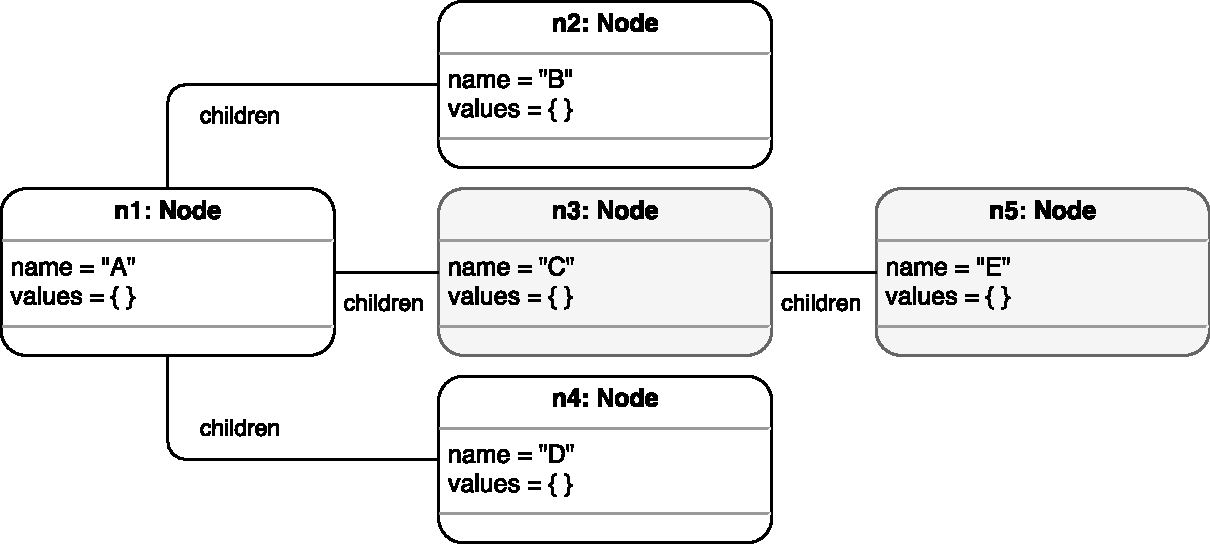
\includegraphics[width=\linewidth]{initial_chart}
\caption{Node \emph{n3} is later deleted from the model.}
\label{fig:initial_model}
	\end{subfigure}
	\caption{A tree metamodel and its model as the running example.}
	\label{fig:append_speed}
\end{figure}

As the first example, we create an tree model as shown in Fig. \ref{fig:initial_model} based on the metamodel in Fig. \ref{fig:node_metamodel}. The model is constructed consisting of three nodes \emph{n1}, \emph{n2}, and \emph{n3}. At first, the three nodes are created and  all operations to set their features are executed. Node \emph{n2} and \emph{n3} are then added to \emph{n1} to contains the other nodes. Later on, node \emph{n3} is deleted from the model. These consecutive operations produce a tree model in List. \ref{lst:xmimodel}.

\noindent
\begin{minipage}[t]{0.34\linewidth}
\begin{lstlisting}[style=xmi,caption={State-based representation of the model in Figure \ref{fig:initial_model} after removal of node \emph{n3} in (simplified) XMI.},label=lst:xmimodel]
<Node id="n1" name="A">
  <children id="n2" 
    name="B"/>
</Node>
\end{lstlisting}
\end{minipage}
\hfill
\begin{minipage}[t]{0.635\linewidth}
\begin{lstlisting}[style=eol,caption={Change-based representation of the model in Figure \ref{fig:initial_model} after removal of node \emph{n3}.},label=lst:cbpmodel]
create n1 of Node
set n1.name to "A"      //n1.name="A"
create n2 of Node
set n2.name to "B"      //n2.name="B"
create n3 of Node
set n3.name to "C"      //n3.name="C"
add n2 to n1.children   //n1.children={n2}
set n2.parent to n1     //n2.parent=n1
add n3 to n1.children   //n1.children={n2,n3}
set n3.parent to n1     //n3.parent=n1
remove n3 from n1.children //n1.children={n2}
delete n3
\end{lstlisting}
\end{minipage}

Instead of treating the model as a state based, we records all events generated by the the consecutive  operations and persist them into a CBP representation (List. \ref{lst:cbpmodel}), which contains at least as much information as the state-based representation. Replaying all these events produces the same state as the one captured in the List. \ref{lst:xmimodel}.  

For a large model, this approach is beneficial since we only need to persist the generated events, not the entire model. However, replaying all the events naively to load the model is not efficient, since unnecessary events are still replayed (unnecessary events are events that are cancelled out by subsequent events). Thus, we propose an algorithm to optimise the loading of the CBP representation. An optimisation can be performed by ignoring the unnecessary events. For example, the deletion of node \emph{n3} makes events (List. \ref{lst:xmimodel}, lines 5-6, 9-12) related to the node unnecessary to be replayed. 

\section{Loading Time Optimisation}
\label{sec:loading_time_optimisation}
The algorithm needs a data structure that memorise objects' events and their position (line number) in a CBP representation so it knows which events that are cancelled out (later on, the line number/the position of an event in a CBP representation is called event number). We call the data structure "model history", a data structure that memorise objects, their events, and their event numbers. Figure \ref{fig:object_history} shows its class diagram.  

\begin{figure}[ht]
\centering
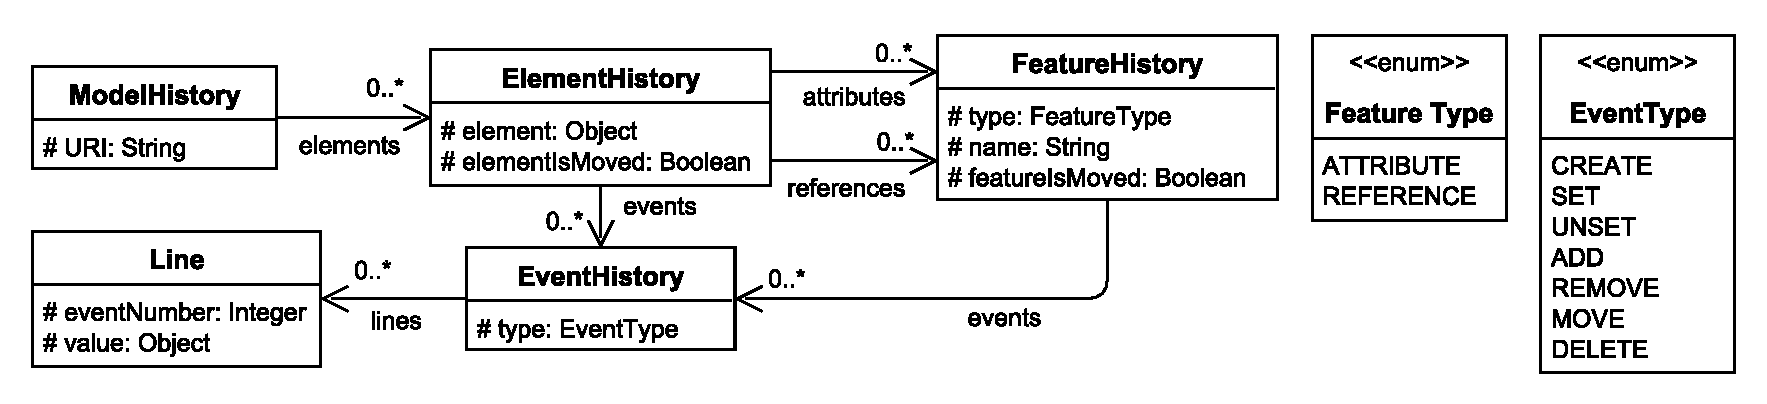
\includegraphics[width=0.8\linewidth]{object_history}
\caption{The class diagram of model history.}
\label{fig:object_history}
\end{figure}

\begin{figure}[ht]
\centering
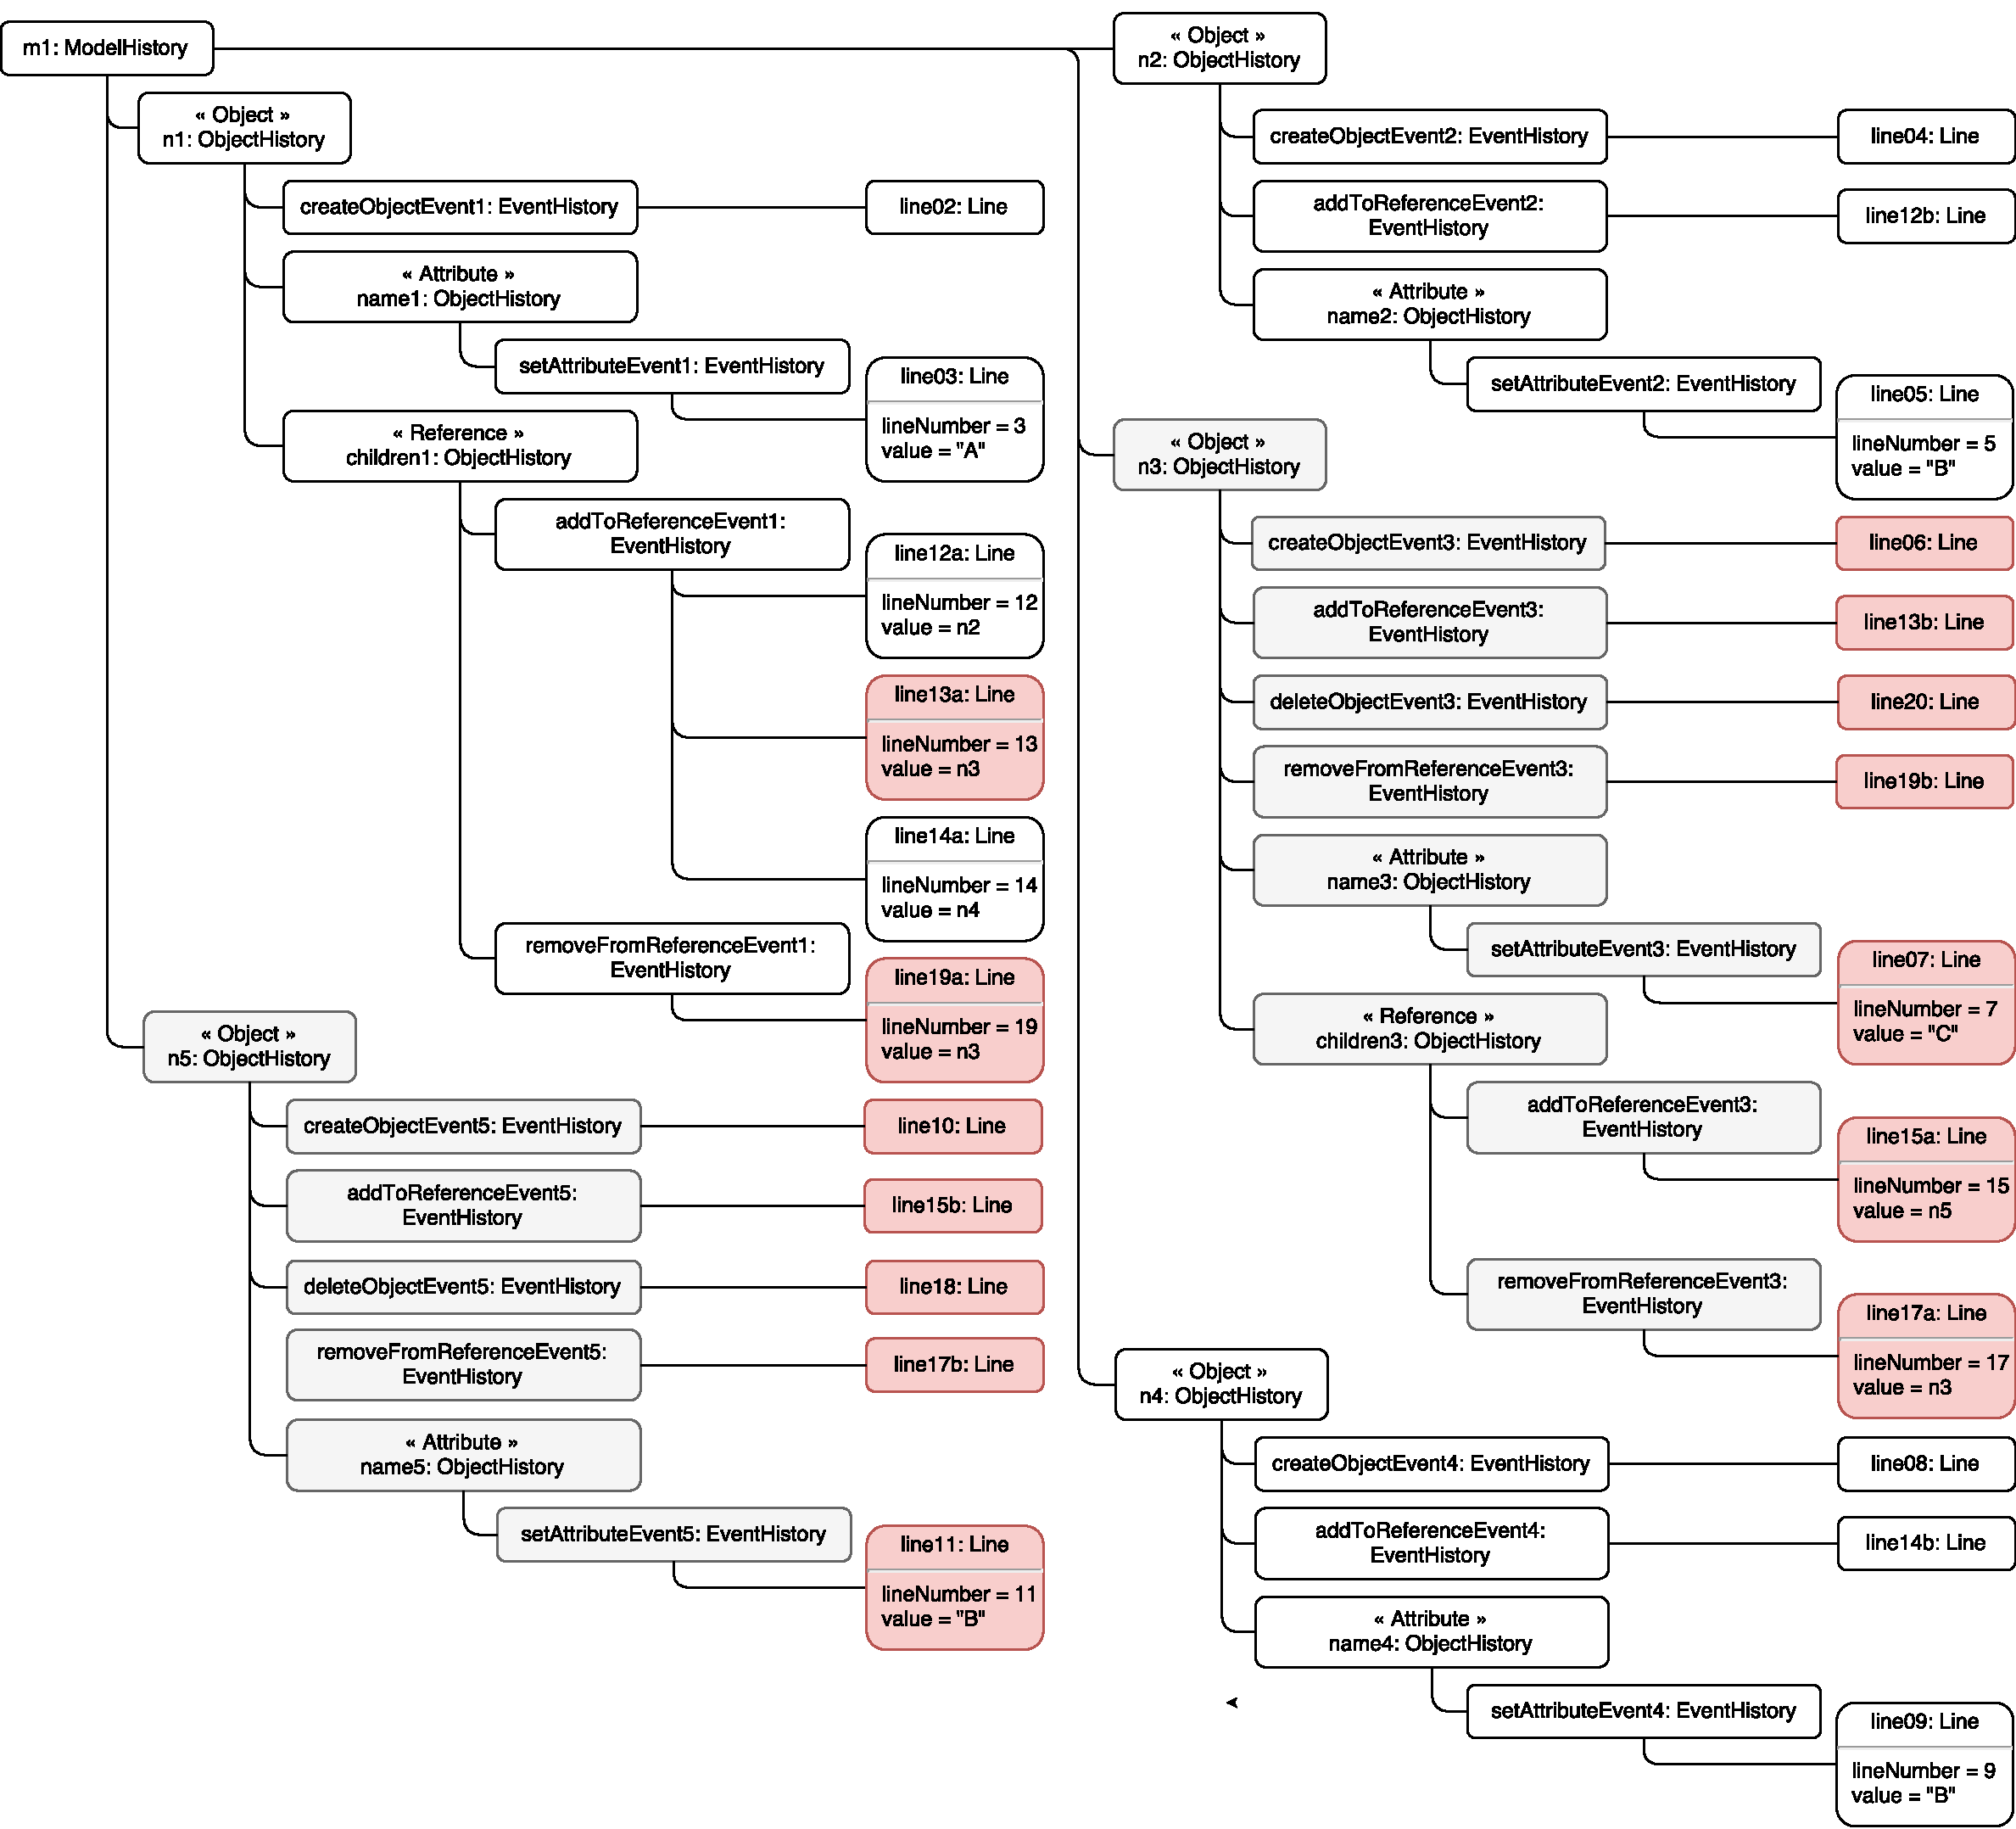
\includegraphics[width=\linewidth]{history_structure}
\caption{The object diagram of model history of the CBP in List. \ref{lst:cbpmodel}.}
\label{fig:history_structure}
\end{figure}

A \emph{ModelHistory} has attribute \emph{URI} to identify the model it records and can have many \emph{ObjectHistory} as its elements. An \emph{ObjectHistory} has an attribute \emph{object} that identify the object that it refers to. The attribute \emph{isMoved} is a flag used to identify the state of the object if the object is already affected by a \emph{move} operation (discussed in subsection \ref{subsec:add_remove_and_move_operations}). Every \emph{ObjectHistory} can have more than one \emph{FeatureStory} to represent features (attribute and reference) that are involved in certain events (i.e. ``\emph{add n2 to n1.children}" event has the \emph{children} as the feature). Each \emph{FeatureStory} can have many \emph{EventHistory} to represent the events. A \emph{FeatureHistory} has two attributes \emph{type} to identify its type, an attribute or reference, and \emph{name} to identify the attribute's name.

There are events that do not involved any feature but only affect objects (i.e. ``\emph{create n1 of Node}" event has no feature involved), or events in which an object acts as an operand for a multi-valued feature (i.e. ``\emph{add n3 to n1.children}" event has the \emph{n3} as the operand). These kinds of events can have their \emph{EventHistory} belong to their \emph{ObjectHistory} directly. An \emph{EventHistory} has an attribute \emph{type} to identify its event type and records a set of \emph{Line}. The \emph{Line} has attributes \emph{eventNumber} and \emph{value} that hold its event number in the CBP representation and the value of involved operand respectively. 

Figure \ref{fig:history_structure} shows the object diagram of model history of the CBP in List. \ref{lst:cbpmodel}. The gray rectangles are objects of \emph{*History} that belong to the deleted node \emph{n3}. The red rectangle indicates objects of \emph{Line} that contains unnecessary event numbers.    

\subsection{Set and Unset Events}
\label{subsec:set_and_unset_events}
During a model development, a single-valued feature can be assigned many times. From all the assignment, only the last assigned value that is necessary for the eventual model---previous assignments can be ignored . For example in List. \ref{lst:set_unset_example}, the attribute \emph{name} is assigned ``A", nullified (unset), and finally ``B". We only need to replay the last assignment (line 4) to produce the same eventual model as if we executes all the operations. 

\noindent
\begin{minipage}[t]{0.49\linewidth}
\begin{lstlisting}[style=eol,caption={The CBP representation of attribute \emph{name} assignments.},label=lst:set_unset_example]
create n1 of Node
set n1.name to "A" //n1.name="A"    
unset n1.name      //n1.name=null
set n1.name to "B" //n1.name="B"
\end{lstlisting}
\end{minipage}
\hfill
\begin{minipage}[t]{0.49\linewidth}
\begin{lstlisting}[style=eol,caption={The CBP representation of reference  \emph{parent} assignments.},label=lst:set_unset_reference]
create n1 of Node
create n2 of Node
create n3 of Node
set n3.parent to n1 //n3.parent=n1
set n3.parent to n2 //n3.parent=n2
unset n3.parent     //n3.parent=null
\end{lstlisting}
\end{minipage}

The event numbers where the attribute \emph{name} affected in Lst. \ref{lst:set_unset_example} are stored into its respective \emph{EventHistory} in \emph{FeatureHistory} in \emph{ObjectHistory}. For example, lines for \emph{set} and \emph{unset} events in their event histories are \emph{setEventHistory.lines = setEventLines =} [[2], [3]] and \emph{unsetEventHistory.lines = unsetEventLines} = [[4]] respectively. Since only the last value of set or unset operations that is significant, using the two lists, we can identify that line 4 is the last line of set and unset operations that is significant for the attribute \emph{name}. Therefore, lines 2 and 3 can be put into an ignore list (\emph{ignoreList} = [2, 3]). The \emph{ignoreList} acts as a lookup reference when a CBP is loaded. If an event's event number is contained in the \emph{ignoreList}, the event is not replayed and the load process continue to the next event.

\begin{algorithm}[H]
\begin{small}
\SetKwInOut{Input}{input}
\SetKwInOut{Output}{output}
\SetKwProg{Struct}{struct}{}{end}
\Struct{Line}{
    Integer $eventNumber$;
    Var $value$;
}
\Input{two lists of Line $setEventLines$ and $unsetEventLines$, a list of Integer $ignoreList$}
\Output{a list of Integer $ignoreList$}
\SetKwBlock{Beginn}{beginn}{ende}
\Begin{
$setLastLine$ $\leftarrow$ getLastLine($setEventLines$)\;
$unsetLastLine$ $\leftarrow$ getLastLine($unsetEventLines$)\;
\uIf{$setLastLine > unsetLastLine$}{
    Add every event number in $setEventLines$ into $ignoreList$ except the last line\;
    Add all event numbers in $unsetEventLines$ into $ignoreList$\; 
}

\ElseIf{$setLastLine < unsetLastLine$}{
    Add all event numbers in $setEventLines$ into $ignoreList$\;
    Add all event numbers in in $unsetEventLines$ into $ignoreList$\; 
}
\Return{$ignoreList$}\;
}
\end{small}
\caption{Algorithm to identify event numbers of unnecessary \emph{set} and \emph{unset} events}
\label{alg:set_unset_optimisation}
\end{algorithm}

The algorithm to execute the rationale is shown in Alg. \ref{alg:set_unset_optimisation}. It works by taking as inputs lists of event numbers of set events (\emph{setEventLines}) and unset events (\emph{unsetEventLines}) of a feature, obtaining the last event numbers between of two lists using function \emph{getLastLine}, and comparing both last event numbers to decide which events numbers that should be put into an ignore list. If \emph{setLastLine} is larger than \emph{unsetLastLine} then all event numbers in both lists can be put into the \emph{ignoreList}, excluding the last value since the last line still need to be replayed to set the value of the feature. If \emph{unsetLastLine} is larger than \emph{setLastLine} then all event numbers in both lists can put the \emph{ignoreList} without exception. The \emph{ignoredList} is then returned for further processes. Listing \ref{lst:set_unset_reference} is another example for reference type of feature. Using the same approach, we can derive that, by the end of the process, \emph{ignoreList} = [4, 5, 6].   

\subsection{Add, Remove, and Move Events}
\label{subsec:add_remove_and_move_operations}
An attribute can also have many values. For example in List. \ref{lst:add_remove_move_attribute},  We add values 11, 12, and 13 subsequently to the attribute \emph{values} and remove the value 12 at line 5  (the commented parts show the states of \emph{node.values}). The replay of the CBP can be optimised by ignoring the add and remove events of the value 12 since we can produce the same eventual model only by adding 11 and 13. To identify that lines 3 and 5 can be ignored, we execute algorithm that is shown in Alg. \ref{alg:add_remove_move_optimisation}.  

\begin{lstlisting}[style=eol,caption={Example of CBP representation of attribute \emph{values}'s add and remove operations.},label=lst:add_remove_move_attribute]
create node of Node
add 11 to node.values      //node.values=[11] 
add 12 to node.values      //node.values=[11,12] 
add 13 to node.values      //node.values=[11,12,13] 
remove 12 from node.values //node.values=[11,13] 
\end{lstlisting}


The algorithm works similar to the algorithm for \emph{set} an \emph{unset} events, except that a feature can contain many values. Therefore, two lists of \emph{Line}---\emph{addEventLines} and \emph{removeEventLines}, excluding \emph{moveEventLines} (the reason for exclusion is explained later)---that it takes as inputs have to be filtered first according to the value that involved in the events using function \emph{filterbyValue}, so that when putting them into the \emph{ignoreList} does not include event numbers for other values (lines 6-7). Lines 8-16 of the algorithm runs similar to the algorithm for \emph{set} an \emph{unset} events. 
 
However, this logics can only be executed if there is no \emph{move} event has been applied to the feature (the reason is explained later in this section) and it is indicated by false value of the flag \emph{featureIsMoved} (line 5). That is why excluding \emph{moveEventLines} is excluded from filtering because no \emph{move} event has been made. The flag \emph{featureIsMoved} is set to true (false is the default value) when the first \emph{move} event is applied to the feature and is set back to false when the feature is empty or has no value. If the feature is empty then all event numbers in the \emph{addEventLines}, \emph{removeEventLines}, and \emph{moveEventLines} into the \emph{ignoreList}. After that, \emph{attributeIsMoved} is set to false. Finally, the \emph{ignoreList} is returned for further operations. Listing \ref{lst:add_remove_move_reference} is another example for reference type of feature for \emph{add} and \emph{remove} events. Using the same approach, we can derive that, by the end of the process, \emph{ignoreList} = [5, 6].       

\begin{algorithm}[H]
\begin{small}
\SetKwInOut{Input}{input}
\SetKwInOut{Output}{output}
\SetKwProg{Struct}{struct}{}{end}
\Struct{Line}{
    Integer $eventNumber$;
    Anytype $value$;
}
\Input{three lists of Line $addEventLines$, $removeEventLines$, and $moveEventLines$, a list of Integer $ignoreList$, a variable of Anytype $operandValue$, a variable of Boolean $attributeIsMoved$, an object of Feature $feature$}
\Output{a list of Integer $ignoreList$}
\SetKwBlock{Beginn}{beginn}{ende}
\Begin{
\If{$featureIsMoved$ = false}{
    $filteredAddLines$ $\leftarrow$ filterByValue($addEventLines$, $operandValue$)\;
$filteredRemoveLines$ $\leftarrow$ filterByValue($removeEventLines$, $operandValue$)\;
$addLastLine$ $\leftarrow$ getLastLine($filteredAddLines$)\;
$removeLastLine$ $\leftarrow$ getLastLine($filteredRemoveLines$)\;
\uIf{$addLastLine > removeLastLine$}{
    Add every event number in $filteredAddLines$ into $ignoreList$ except the last value\;
    Add all event numbers in $filteredRemoveLines$ into $ignoreList$\; 
}
\ElseIf{$addLastLine < removeLastLine$}{
    Add all event numbers in $filteredAddLines$ into $ignoreList$\;
    Add all event numbers in $filteredRemoveLines$ into $ignoreList$\; 
}
}
\If{feature is empty}{
        Add all event numbers in $addEventLines$, $removeEventLines$, and $moveEventLines$ into $ignoreList$\;
        $attributeIsMoved$ $\leftarrow$ false\;
}
\Return{$ignoreList$}\;
}
\end{small}
\caption{Algorithm to identify event numbers of unnecessary \emph{add}, \emph{remove}, and \emph{move} events.}
\label{alg:add_remove_move_optimisation}
\end{algorithm}

\begin{lstlisting}[style=eol,caption={Example of CBP representation of attribute \emph{values}'s add and remove operations.},label=lst:add_remove_move_reference]
create n1 of Node
create n2 of Node
create n3 of Node
add n2 to n1.children      //n1.children=[n2] 
add n3 to n1.children      //n1.children=[n2,n3] 
remove n3 from n1.children //n1.children=[n2] 
\end{lstlisting}

The flag \emph{featureIsMoved} at line 5 in Alg. \ref{alg:add_remove_move_optimisation} is required to prevent error when replaying a CBP that already optimised. If the feature has been applied a move event that move a certain value based on defined \emph{from} and \emph{to} indexes, ignoring previous events can place a value that is different from the unoptimised CBP on the defined \emph{from} index. Thus, replaying the optimised CBP can produce an eventual model that is different from the unoptimised one. For example, when replaying List. \ref{lst:move_attribute_example_error}, the optimised CBP of List. \ref{lst:move_attribute_example}, it produces \emph{node.values} = [13, 11], which is different from \emph{node.values} = [11,13]  that is produced from replaying original CBP, since ``\emph{add 12 to node.values}" and ``\emph{remove 12 from node.values}" events are already excluded in the optimisation process if there is no flag \emph{featureIsMoved} that prevents the exclusion.


\begin{lstlisting}[style=eol,caption={The CBP representation of attribute \emph{values}'s move event.},label=lst:move_attribute_example]
create node of Node
add 11 to node.values            //node.values=[11] 
add 12 to node.values            //node.values=[11,12] 
add 13 to node.values            //node.values=[11,12,13] 
move from 0 to 1 in node.values  //node.values=[12,11,13]  
remove 12 from node.values       //node.values=[11,13] 
\end{lstlisting}

\begin{lstlisting}[style=eol,caption={The optimised CBP representation of attribute \emph{values}'s event.},label=lst:move_attribute_example_error]
create node of Node              //(1)  
add 11 to node.values            //(2) node.values=[11] 
add 13 to node.values            //(4) node.values=[11,13] 
move from 0 to 1 in node.values  //(5) node.values=[13,11]   
\end{lstlisting}

\subsection{Create and Delete Events}
\label{subsec:create_and_delete_operations}
While \emph{create} event has been demonstrated in almost every Listing in this paper, \emph{delete} event is demonstrated in Lst. \ref{lst:cbpmodel}. When an object is deleted, it means that the object is completely removed from the model. Therefore, all events (create, set, unset, move, add, remove, delete) related to the object can be ignored, including all events related to its features. For example, when node \emph{n3} in Lst. \ref{lst:cbpmodel}  in the first example is deleted, replaying lines 5-6 and 9-12 is unnecessary and therefore the event numbers of the lines can be put into \emph{ignoreList} producing \emph{ignoreList} = [5, 6, 9, 10, 11, 12]. The optimised CBP of List. \ref{lst:cbpmodel} is presented in List. \ref{lst:cbpmodel_optimised}. The numbers that are in the brackets in the commented parts are the lines' previous event numbers in the unoptimised CBP.  

\begin{lstlisting}[style=eol,caption={Change-based representation of the model of Figure \ref{fig:initial_model} after removal of node \emph{n5}.},label=lst:cbpmodel_optimised]
create n1 of Node       //(1)
set n1.name to "A"      //(2) n1.name="A"
create n2 of Node       //(3)
set n2.name to "B"      //(4) n2.name="B"
add n2 to n1.children   //(7) n1.children={n2}
set n2.parent to n1     //(8) n2.parent=n1
\end{lstlisting}

We use Alg. \ref{alg:create_delete_optimisation} to determine lines that are ignored after a \emph{delete} event. The algorithm
works by iterating through all the \emph{EventHistory} of all its {FeatureHistory} and all its direct {EventHistory}, and putting all the event numbers found into the \emph{ignoreList}.

The algorithm starts by checking flag \emph{objectIsMoved} to determine whether the \emph{deletedObject} is already moved or not (line 2). If it is false then it is safe to remove all lines that refer to the object (line 3) (the reason for use of the flag has been explained in subsection \ref{subsec:add_remove_and_move_operations}). Otherwise, no action is executed. The algorithm then retrieves all event histories \emph{eventHistoryList} that refer to the object (line 4) and iterates through each event history (line 5-8). For every event history \emph{eventHistory} (line 5), the algorithm retrieves its lines \emph{lineList} (line 6) and put all their event numbers into the \emph{ignoreList} (line 7). After that, the algorithm continues to iterate through all its features and put all lines' event numbers of their events into the \emph{ignoreList} (lines 12-15). Finally, the algorithm returns the \emph{ignoreList} as its output.

\begin{algorithm}[H]
\begin{small}
\SetKwInOut{Input}{input}
\SetKwInOut{Output}{output}
\Input{a variable ofObject $deletedObject$, a list of Integer $ignoreList$}
\Output{a list of Integer $ignoreList$}
\Begin{
$objectIsMoved$ $\leftarrow$ isObjectMoved($deletedObject$)\;
\If{$objectIsMoved$ = false}{
    $eventHistoryList$ $\leftarrow$ getAllEventHistories($deletedObject$)\; 
    \ForEach{$eventHistory$ in $EventHistoryList$}{
        $lineList$ $\leftarrow$ getLines($eventHistory$)\;
        Add all event numbers in $lineList$ into $ignoreList$\; 
    }
    $featureList$ $\leftarrow$ getAllAttributes($deletedObject$)\;
    \ForEach{$attribute$ in $featureList$}{
        $eventHistoryList$ $\leftarrow$ getAllEventHistories($feature$)\;
        \ForEach{$eventHistory$ in $EventHistoryList$}{
            $lineList$ $\leftarrow$ getLines($eventHistory$)\;
            Add all event numbers in $lineList$ into $ignoreList$\; 
        }       
    }   
}
\Return{$ignoreList$}\;
}
\end{small}
\caption{Algorithm to identify lines that are ignored after \emph{delete} events}
\label{alg:create_delete_optimisation}
\end{algorithm}



\section{Performance Evaluation}
\label{sec:performance_evaluation}
We have implemented a prototype\footnote{The prototype is available under [hidden for review] %\url{https://github.com/epsilonlabs/emf-cbp}
} of the change-based model persistence using the Eclipse Modelling Framework. We evaluate the prototype's performance on saving time, loading time, and memory consumption. For the saving time, we contrast the saving time between optimised CBP, unoptimised CBP, and XMI. For the loading time, we perform comparison on loading time between optimised CBP, non-optimised CBP, and XMI. For memory consumption, we compare the performance of optimised CBP and XMI on memory consumption. The evaluation is performed on Windows Server 2008 R2 64-bit with processor Intel Xeon E5530 @2.40 GHz (2 processors) and memory 36 GB.

\begin{figure}[htbp]
    \centering
    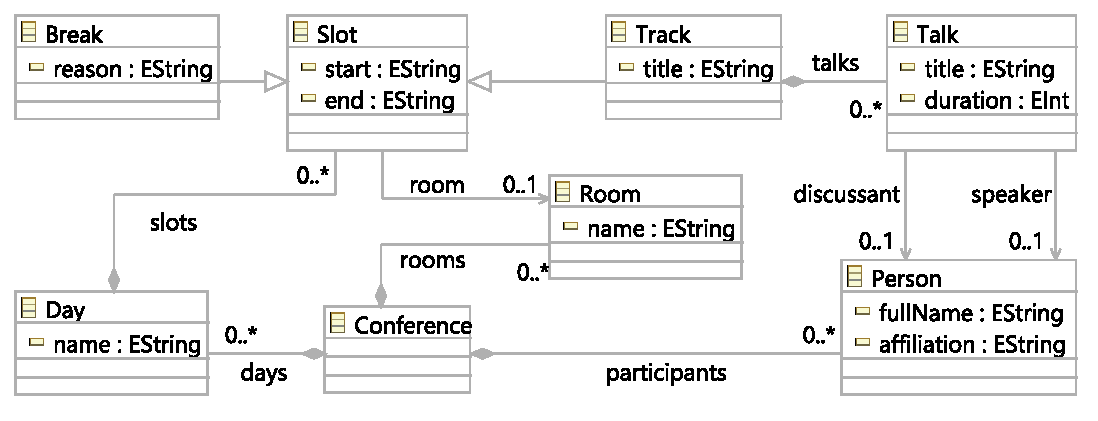
\includegraphics[width=0.9\linewidth]{conference_metamodel}
    \caption{A conference metamodel.}   
    \label{fig:node_metamodel}
\end{figure}

In the evaluation, we introduce conference model to evaluate the optimisation closer to the real-world problem since the tree domain in our examples is trivial and not common used in the real-world. The conference model covers more of EMF features; it has more than one class (Conference, People, Room, etc. classes) and it applies inheritance. Figure \ref{fig:node_metamodel} shows its metamodel. 

\subsection{Saving Time}
\label{subsec:saving_time_test}
We evaluate the performance of our prototype on saving time to gain insight on the efficiency that can be gained from the optimised CBP against the unoptimised CBP and XMI as the comparison baselines. The comparison is depicted in Fig. \ref{fig:append_speed}.

We seek the relationship between number of objects in a model and the time required to persist the model. We create courses of random operations in Epsilon Object Language \cite{kolovos2006epsilon} for each tree and conference domains and executed them to simulate the development of models. In the random operations, we set the probability of different types (create, set, unset, add, move, delete) of operations to occur to 10:1:1:1:1:1 respectively. For the conference model, since it has several classes (Person, Day, Room, Break, Track, Talk), we set ratio 40:1:3:6:8:24 respectively for them to be created in the \emph{create} operation to ensure that the model is generated proportionally. Along the growing of the model, we count the number of the objects. Every increase in 100 objects, we measure the time. For  the optimised and unoptimised CBPs, we measure the time consumed to append events generated for each operation, while for XMI, we measure the time used to persist the eventual state of the model after each operation. 

\begin{figure}[ht]	
	\begin{subfigure}[t]{0.5\linewidth}
		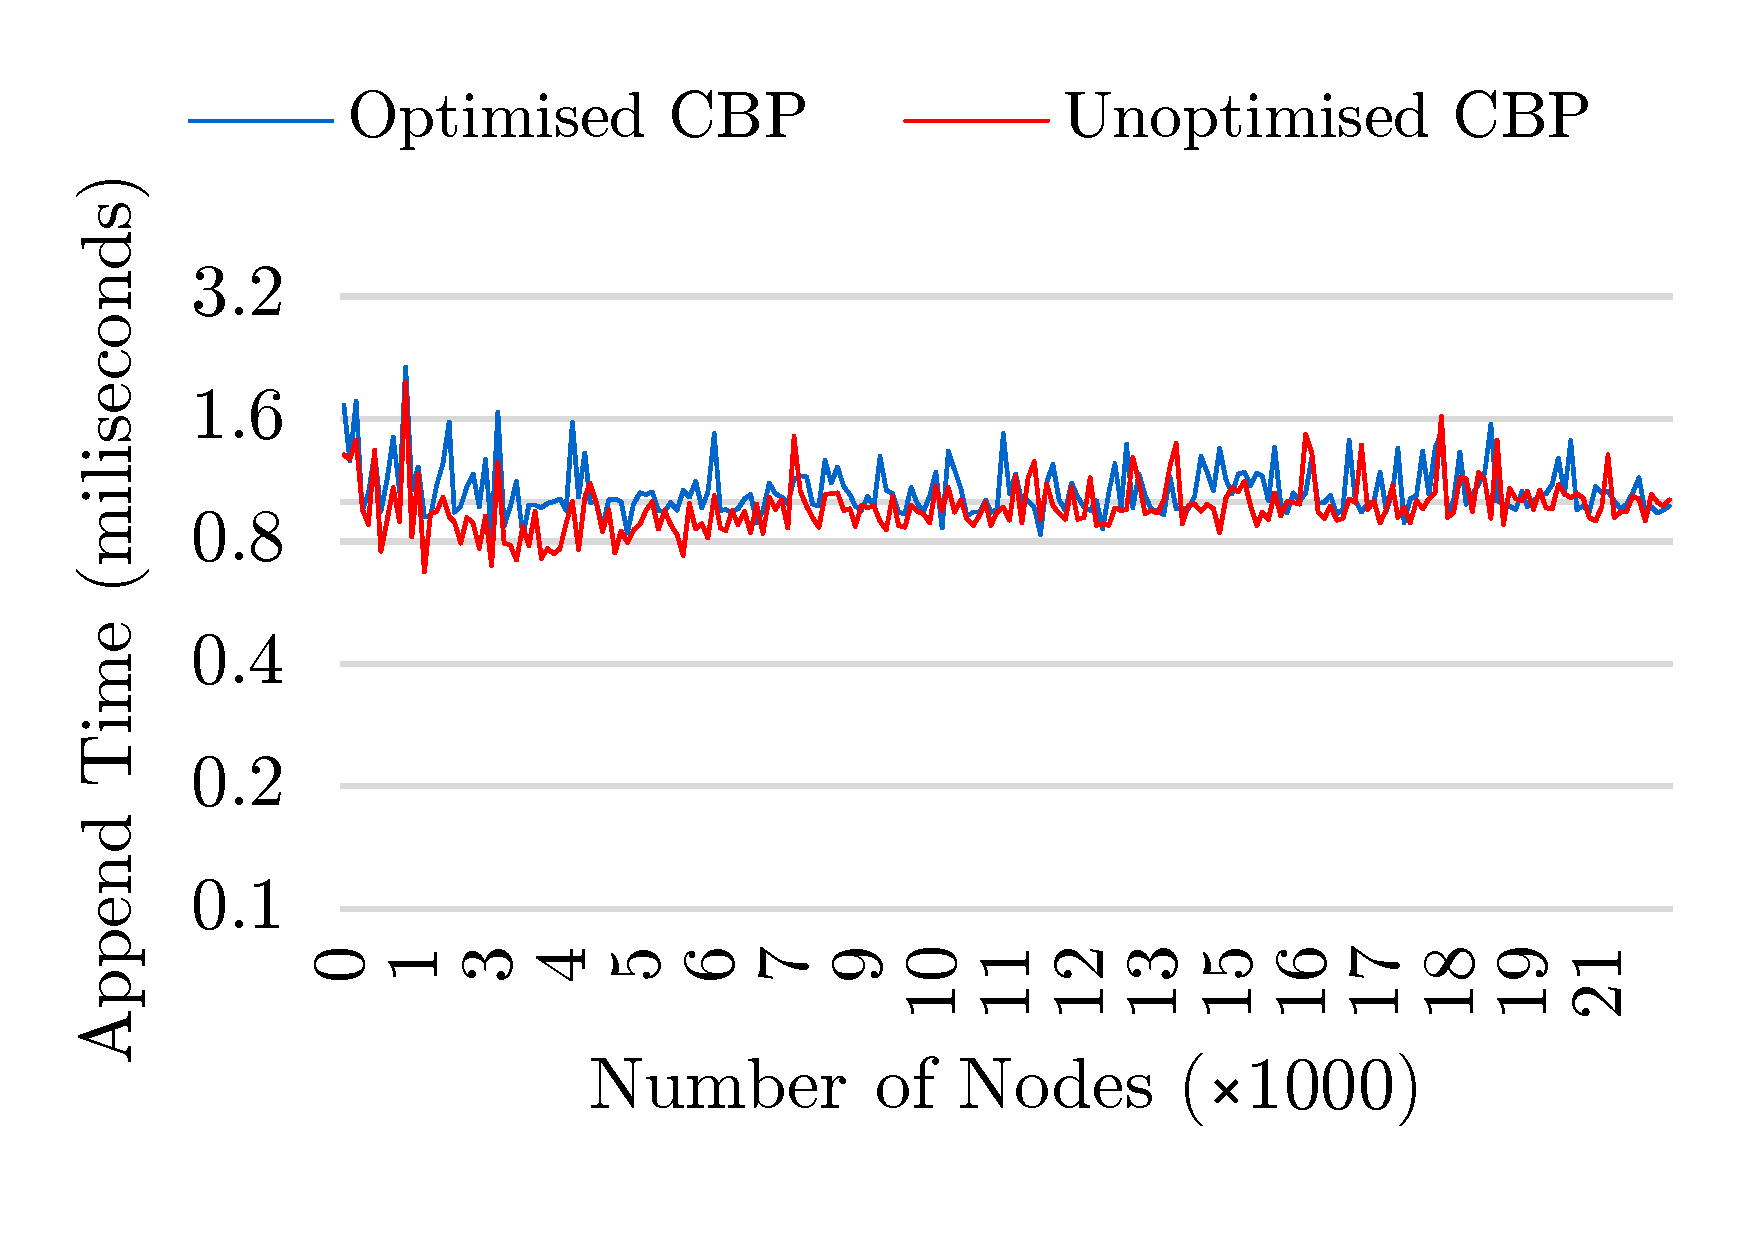
\includegraphics[width=\linewidth]{append_speed_tree}
		\caption{Tree domain}\label{fig:append_speed_tree}		
	\end{subfigure}
	\hfill
	\begin{subfigure}[t]{0.5\linewidth}
		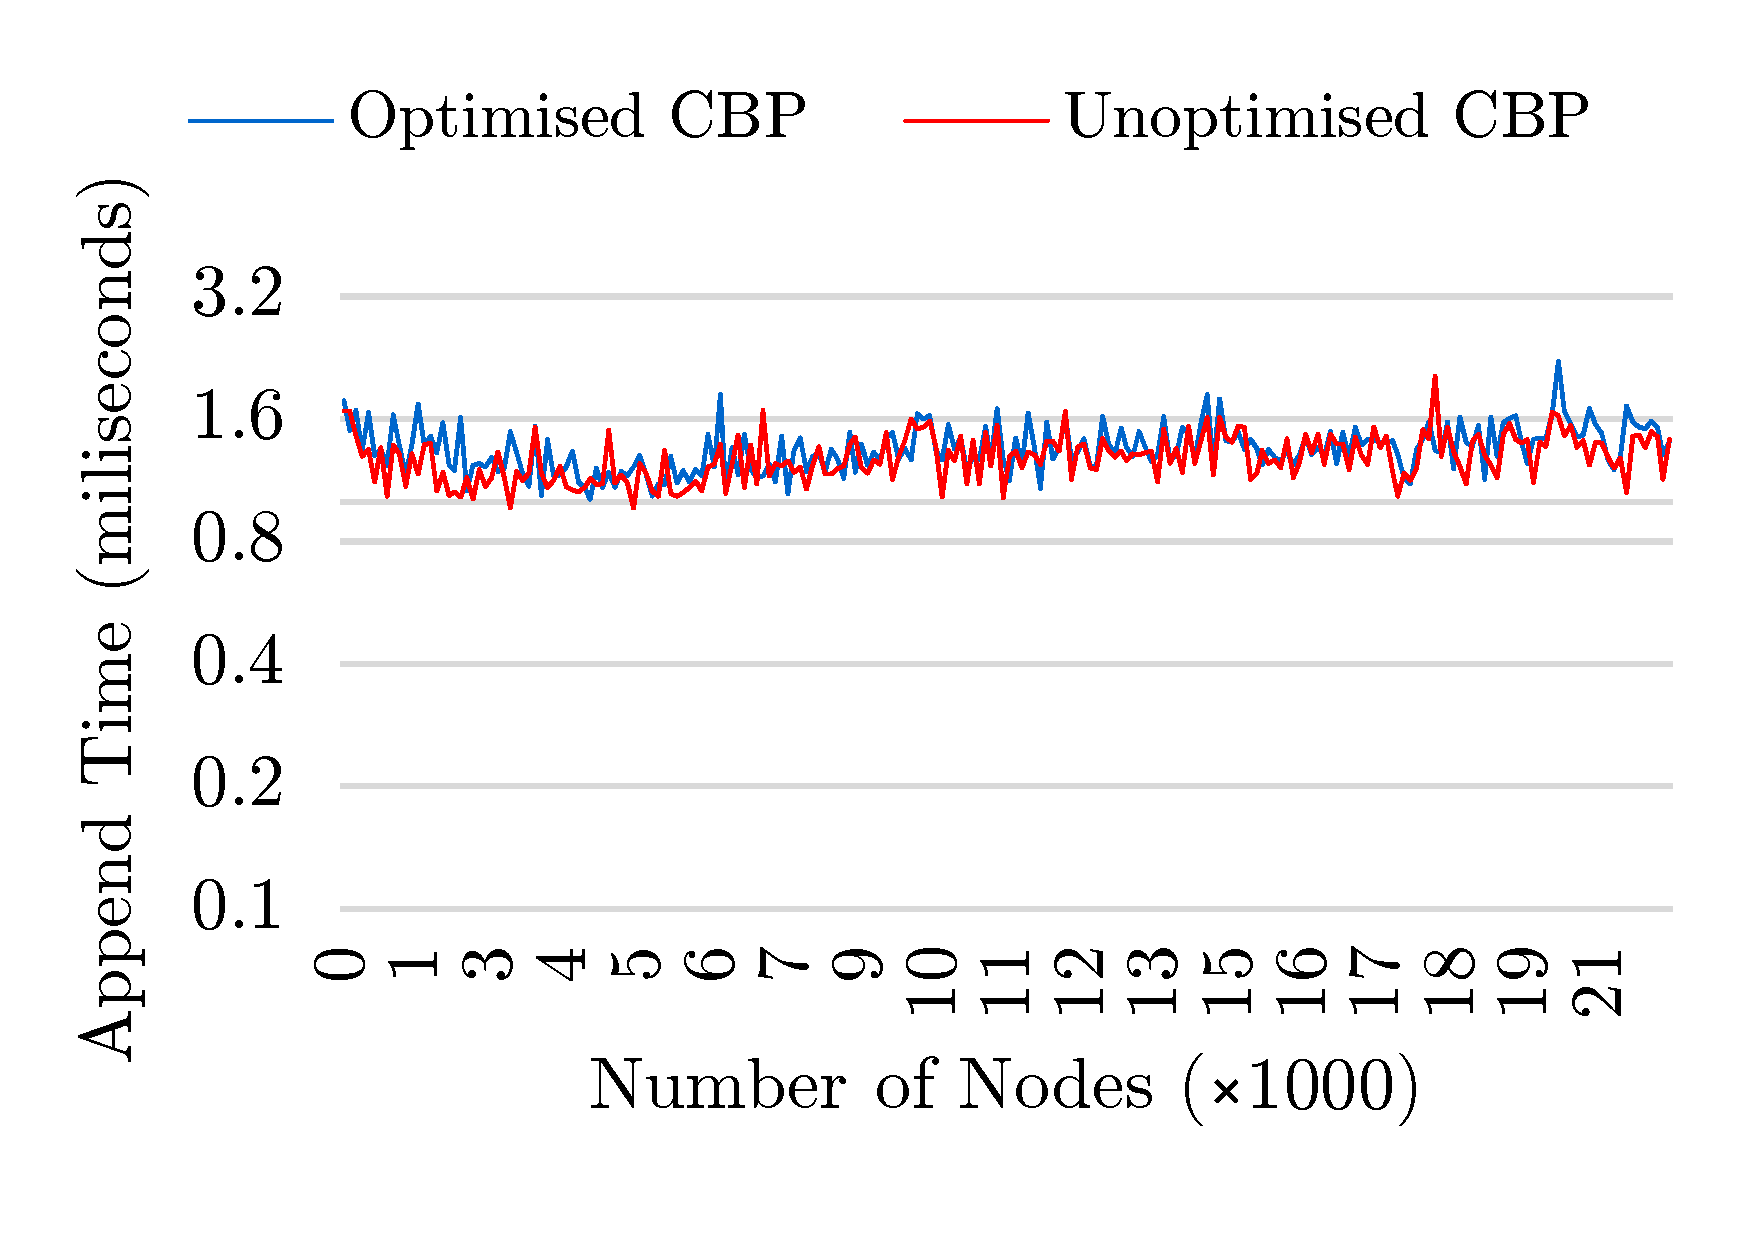
\includegraphics[width=\linewidth]{append_speed_conf}
		\caption{Conference domain}\label{fig:append_speed_conference}
	\end{subfigure}
	\caption{A comparison on time used to persist models between CBP and XMI. The y-axis is log\textsc{2} scaled.}
	\label{fig:append_speed}
\end{figure}

In Fig. \ref{fig:append_speed}, for both tree and conference domains, the time consumed to persist events in both CBPs is nearly constant, whereas for XMI, the time consumed to persist a model increases linearly along the growth of objects (its graph is not displayed since it is outperformed by both CBPs). The append time of optimised CBP is slightly slower than the unoptimised CBP's since it has additional computation to populate the \emph{ModelHistory} and \emph{IgnoreList}. Based on our measurement, the average time consumed to append events into a CBP representation is 1.16 miliseconds, and the time to save model in XMI is increased 2.25 microseconds for each additional object. This finding suggests persisting changes of a model is significantly faster than persisting its complete eventual state after the model is modified.    

\subsection{Loading Time}
\label{subsec:loading_time_test}
We compare optimised CBP, non-optimised CBP, and XMI on their loading time to evaluate the performance of the optimisation algorithm. The  comparison is depicted in Fig. \ref{fig:loading_speed}. We seek the relationship between number of objects of a model and time required to load the model. We create courses of random operations and execute them to simulate the model construction.   

In performing the simulation, we create generate a number of random operations (create, set, unset, add, move, delete) to manipulate the objects. The number of the random operations is as many as the number of the initial objects. Also, the probability of the different types of operations to occur is set to 1:1:1:10:5:1. For each iteration, we increase the number of initial objects and the random operations each by 500. For conference model, since it has several classes (Person, Day, Room, Break, Track, Talk), we set ratio 40:1:3:6:8:24 respectively for them to be created in the initial objects and \emph{create} operation to ensure that the model is generated proportionally. For CBP, we measure the time consumed to append events generated for every operation. For XMI, we measure the time used to persist the eventual state for each model generated.

\begin{figure}	
	\begin{subfigure}[t]{0.5\linewidth}
		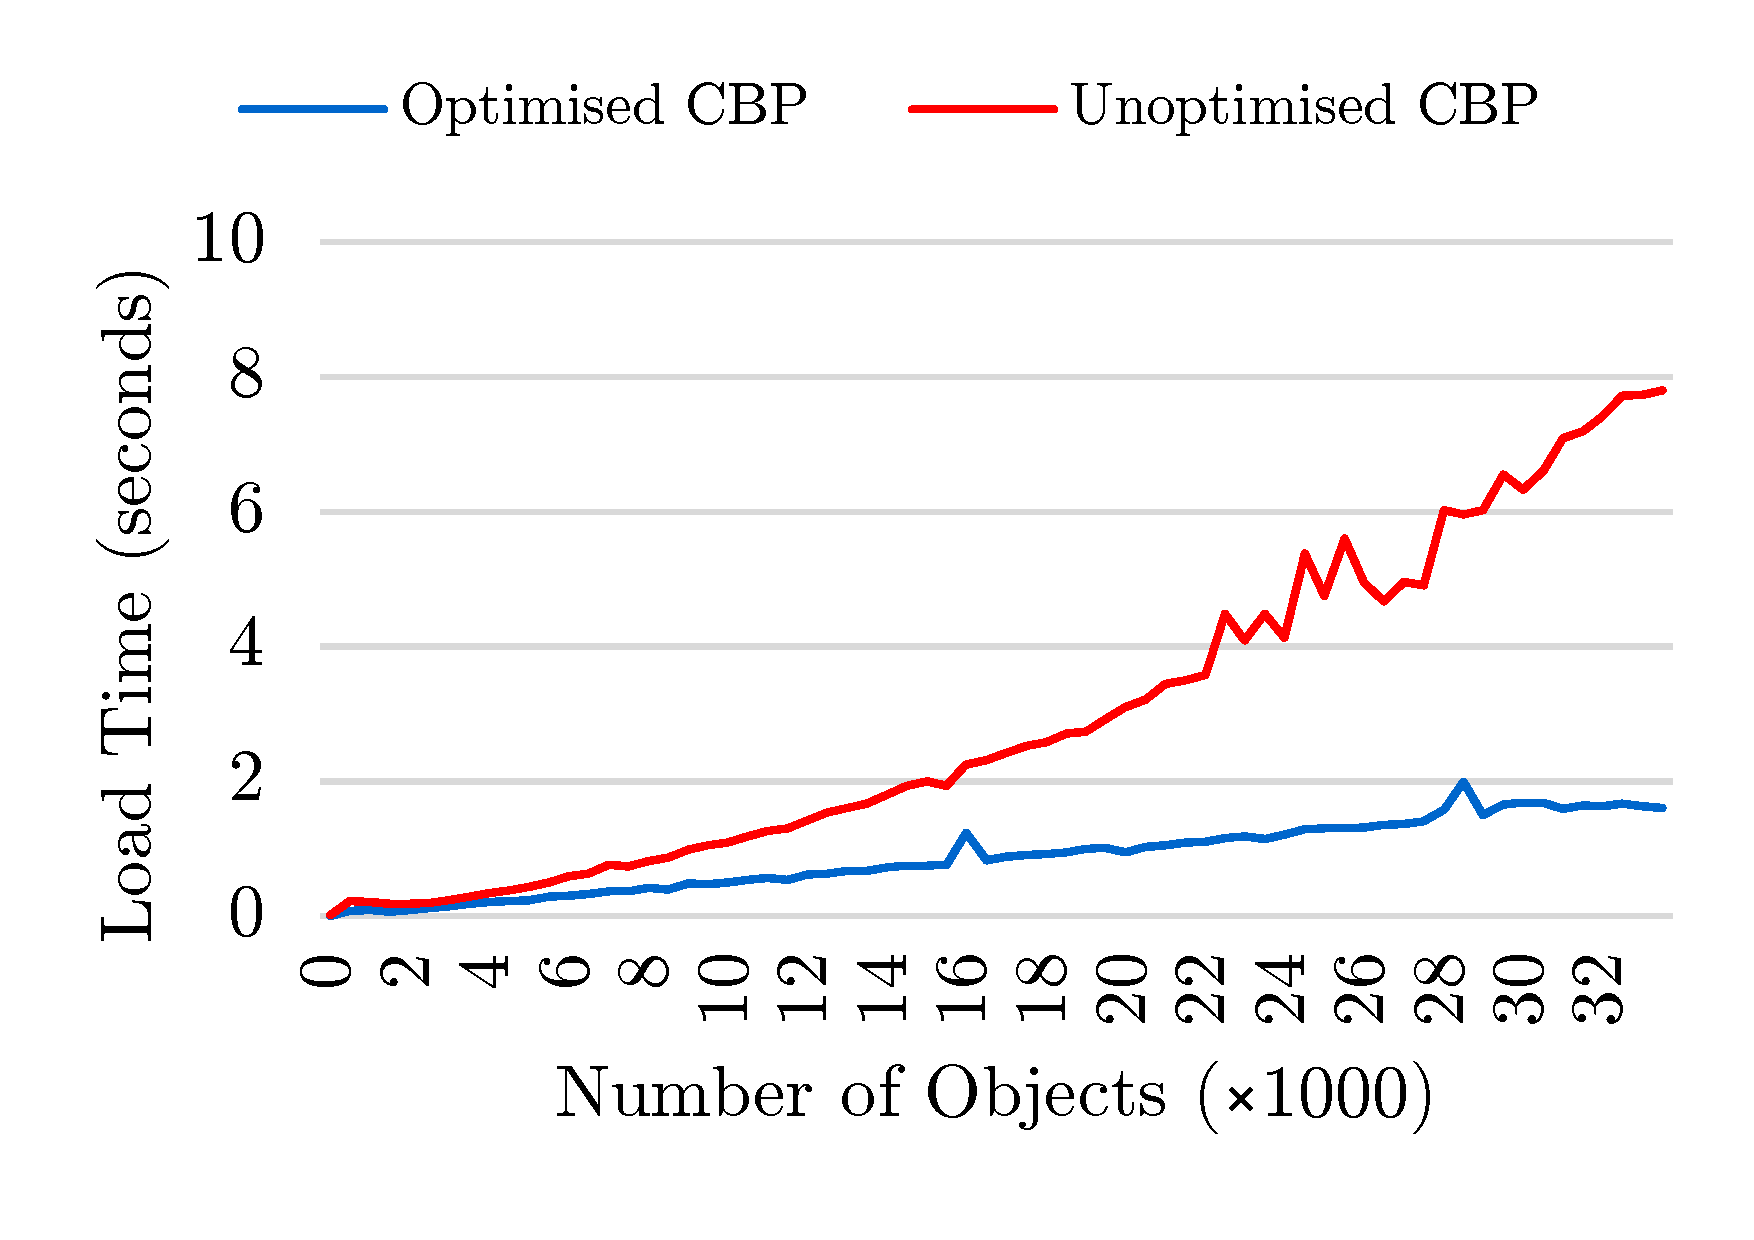
\includegraphics[width=\linewidth]{loading_speed_tree}
		\caption{Tree domain}\label{fig:append_speed_tree}		
	\end{subfigure}
	\hfill
	\begin{subfigure}[t]{0.5\linewidth}
		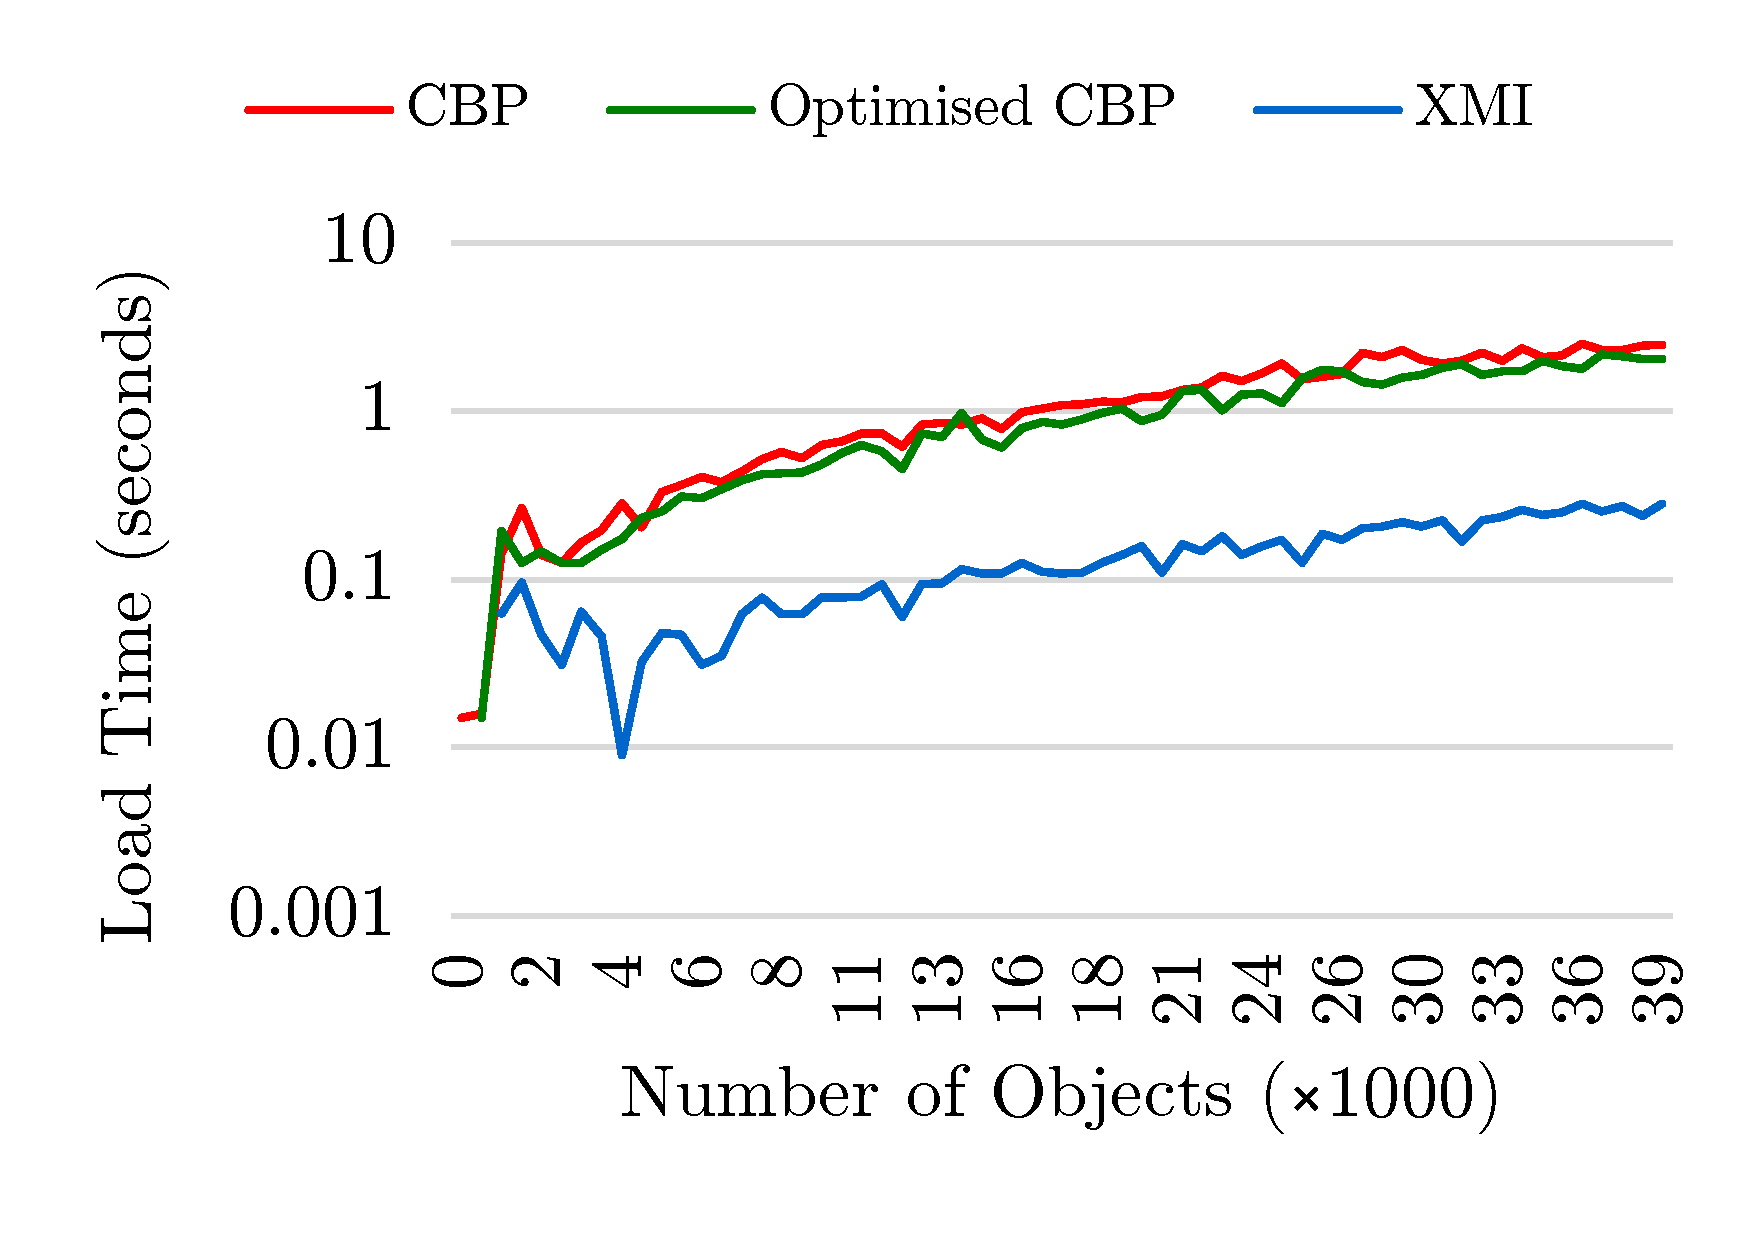
\includegraphics[width=\linewidth]{loading_speed_conf}
		\caption{Conference domain}\label{fig:append_speed_conference}
	\end{subfigure}
	\caption{A comparison on load time between XMI, optimised CBP, and non-optimised CBP. The y-axis is log\textsc{10} scaled.}
	\label{fig:loading_speed}
\end{figure}

Fig. \ref{fig:loading_speed} shows a pattern that the optimised CBP consumes less time than the non-optimised CBP on loading models. However, different domains of models show different efficiency. In the case of conference domain, the optimised CBP's loading time is less efficient than the one in tree domain, even though it is still faster than the non-optimised CBP. Thus, the efficiency depends on the characteristics of the domain's model. We argue that domains that typically perform lots of modifications and deletions will benefit more, such as the tree domain that has multiple levels of containment, which means deleting a node also deleting its direct and indirect nodes, whereas in conference domain, it typically contains hundreds of participants but less likely to have multilevel containment creating a shallow, flat tree-like characteristic. 

In the case of tree model, the optimised CBP is becoming more efficient than the non-optimised CBP when the number of loaded objects is increasing. The optimise CBP's loading time is linearly increasing while the non-optimised one tends to grow exponentially. However, still, it cannot outperform the XMI's loading time, since more time is used to de-serialise the CBP format. Optimising the serialised format will reduce the loading time of the optimised CBP.  

\subsection{Memory Consumption}
\label{subsec:memory_consumption}

\begin{figure}	
	\begin{subfigure}[t]{0.5\linewidth}
		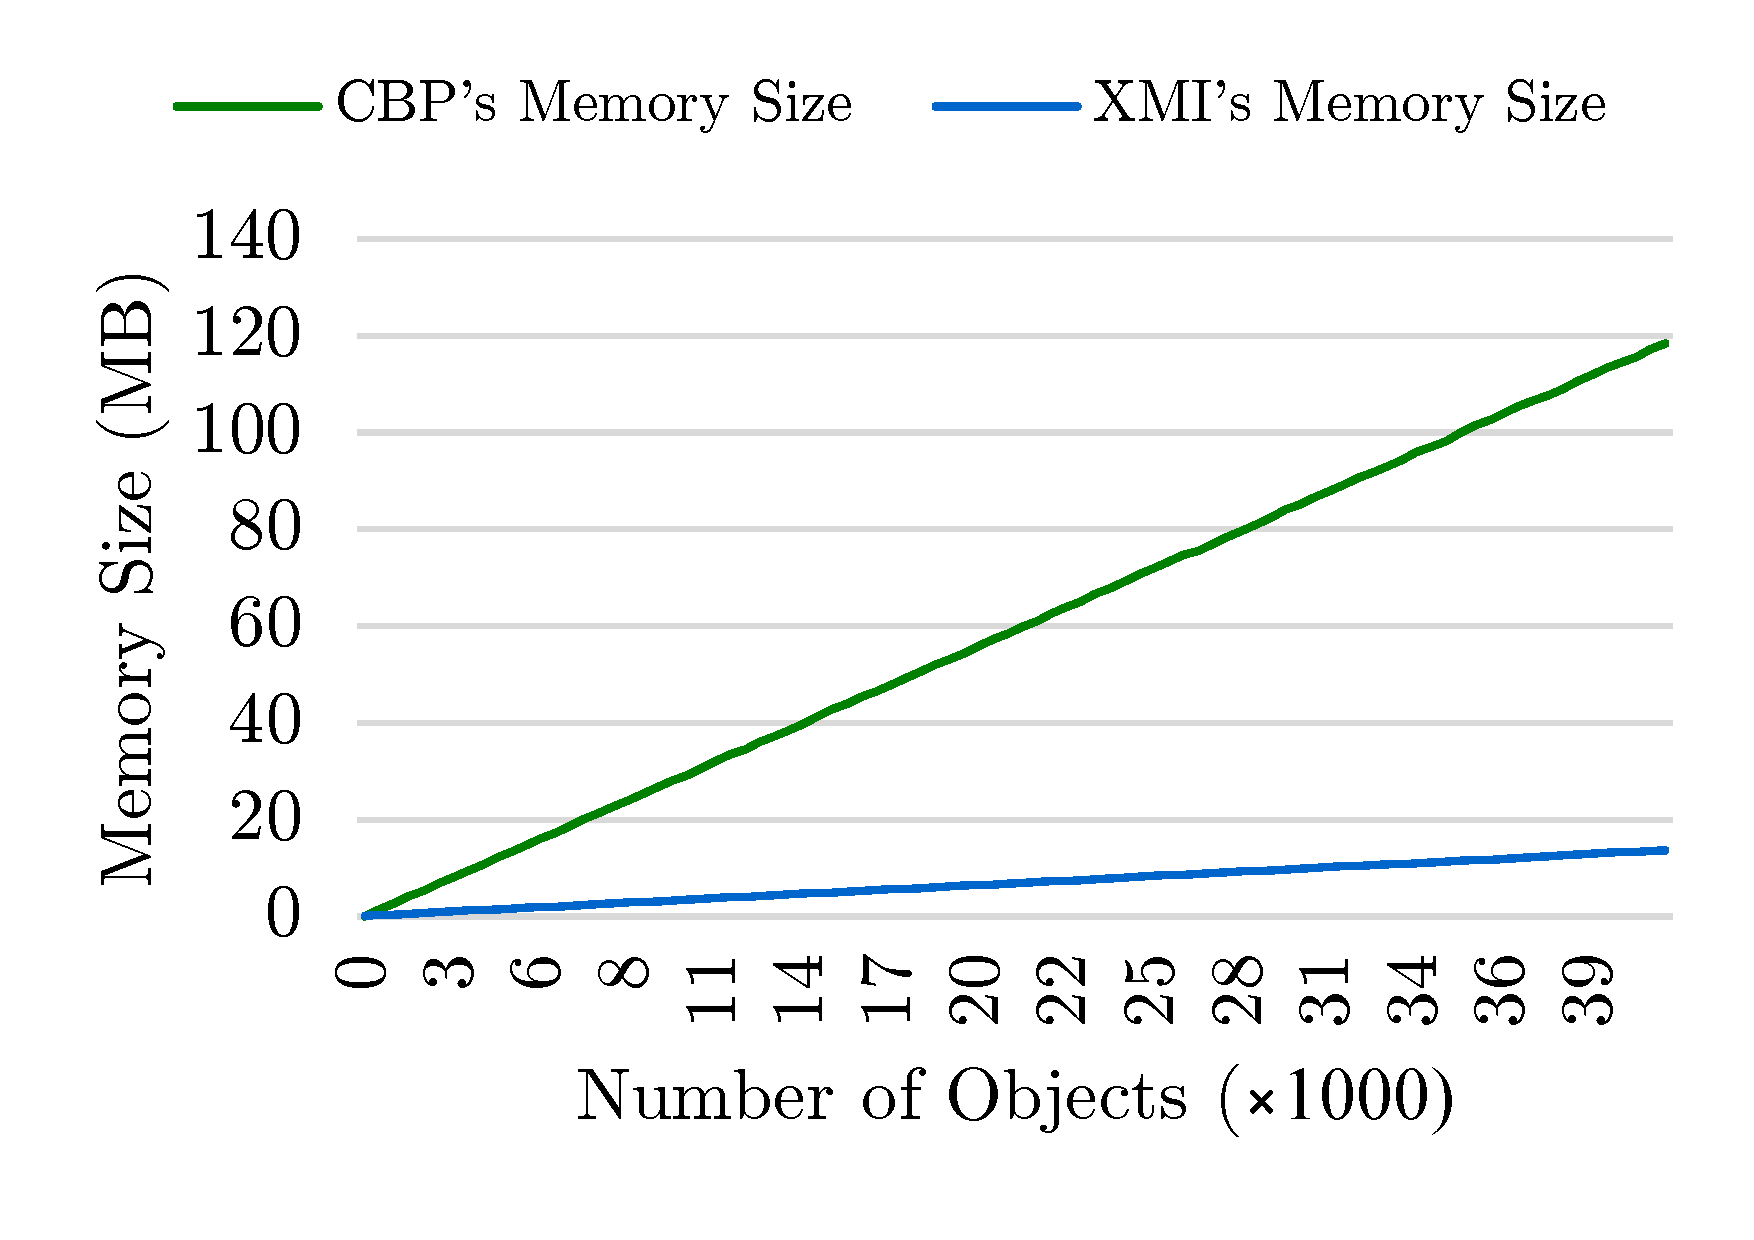
\includegraphics[width=\linewidth]{memory_use_tree}
		\caption{Tree domain}\label{fig:append_speed_tree}		
	\end{subfigure}
	\hfill
	\begin{subfigure}[t]{0.5\linewidth}
		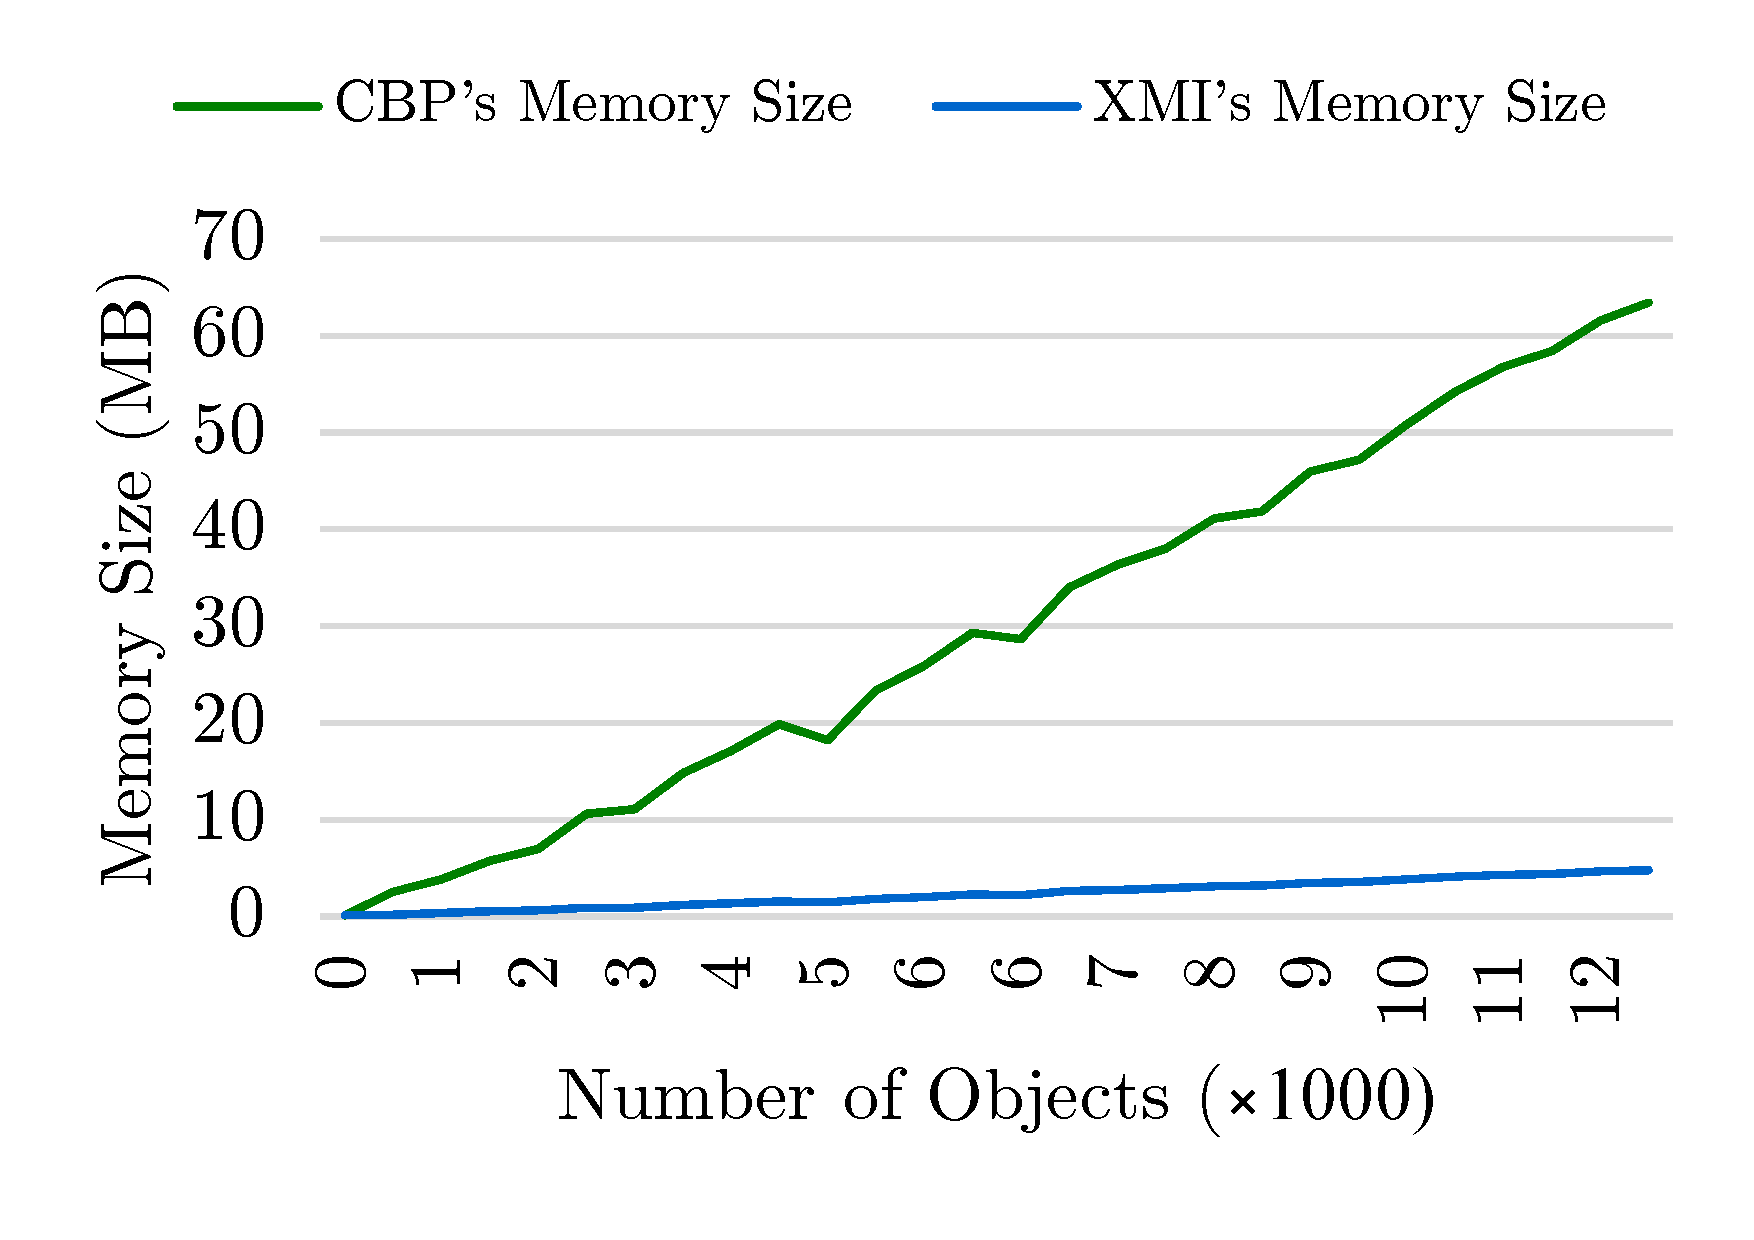
\includegraphics[width=\linewidth]{memory_use_conf}
		\caption{Conference domain}\label{fig:append_speed_conference}
	\end{subfigure}
	\caption{A comparison on memory consumption between CBP and XMI.}
	\label{fig:memory_use}
\end{figure}

Another evaluation that we perform is we optimised CBP and XMI on their memory consumption after loading models. We use the Jamm \cite{brosius2017jamm}, a tool that uses Java agent for memory measurement. It turns out that the results are not significantly different and still follow the same trend). We use a deep measure, every object referenced in the measured object is also calculated, to calculate the total consume. 

The results are shown in Figure \ref{fig:memory_use}. In both tree and conference domains, XMI significantly outperforms CBP in terms of memory consumption after loading models. The large memory consumption of CBP is caused by the model history that consumes space in memory to holds objects, their events, and their event numbers. This condition leads us to another future work that is to identify and remove objects, events, and events numbers from the model history once they are not any longer required. For example, once a object is deleted from a model, all its records in the model history are removed to release space in memory. 

\section{Related Work}
\label{sec:related_work}
Several works have been done in persisting large models , and most of them use databases (e.g. relational, NoSQL). Connected Data Objects (CDO) \cite{eclipse2017cdo} and EMF Teneo \cite{eclipse2017teneo} reduces resources and the time needed to parse XMI documents by persisting models into relational databases. This approach uses metamodels to generate the relational schemas of models and provides  high-level abstraction API for developers to interact with the databases but has drawbacks due to the expensive joins of many tables for highly interrelated models \cite{barmpis2014evaluation}.    
Morsa \cite{pagan2011morsa} uses MongoDB \cite{mongodb2017what}, a NoSQL database, to persist models as a collection of documents by storing every element of a model and its metamodel as entries in an index document that refer to the root objects of their documents. However, due to the nature of the document-based database, storing model's references as serialised documents limits its query and insertion performance as large models have many references which makes them highly interrelated \cite{barmpis2014evaluation}. NeoEMF \cite{daniel2016neoemf} is a prototype that uses several types of NoSQL databases to persist models and lazy-loading mechanism to improve accessing, loading, and removing model elements. Nevertheless, it has not addressed the issues of collaboration, versioning, and fast model differencing. EMFStore \cite{koegel2010emfstore} is a version control system (VCS) that stores changes of models as operations applied to the models, which facilitates collaboration and identify changes of models easier. However, support to use its operation-based approach with more common VCSs (e.g. GitHub, SVN) is not yet available. Several papers mention it does not scale \cite{pagan2011morsa,kolovos2013research} and no optimisation has been proposed to arrive at the eventual versions of models, except replaying all stored operations. 

\section{Limitations}
\label{sec:limitations}
So far, we only address attribute or reference that can only contains unique members---no duplicate values or objects. Duplicate members means that removal of a value /object does not mean the removal of other same values/objects since values/objects with different positions contained in the feature are perceived different. Therefore, positions of values/objects have to be considered by the optimisation algorithm. Furthermore, we also have not addressed features that has default values. Default value of a feature might not trigger any event. Failure to address this might produce different end models. 

Models in the real world are most likely different from the random models generated in the evaluation. Their optimised CBP's loading time can perform better or worse than the ones presented in this paper. In another condition, the optimised CBP is not always outperform the non-optimised CBP in every condition. There is a condition where optimised CBP is not faster than the non-optimised CBP that is when only \emph{create} operation is performed, without performing other types of operation, since there is no event that can be ignored. One feasible way to better reflect real-world models is to ask modellers to create complex models using different modelling languages, persist their histories, and analyse the results to gain insight whether the optimisation really works for real-world models. 

\section{Conclusions}
\label{sec:conclusions}
In this paper, we have proposed a change-based, as an alternative to stated-based, persistence as an approach to persist a model. We also have proposed the algorithm to optimise its loading time as well evaluated the change-based persistence on saving time, loading time, and memory time against the XMI and non-optimised CBP as the baselines. Our results show considerable savings in terms of persisting and identifying changes made to models at an increased---but linear---model loading cost. For future work, we  plan to extend the CBP to enable change detection, model merging, conflict resolution of models in the context of collaborative modelling.

%\subsubsection*{Acknowledgments.} This work was partly supported through a scholarship managed by \emph{Lembaga Pengelola Dana Pendidikan Indonesia} (Indonesia Endowment Fund for Education).

\bibliography{references} 
\bibliographystyle{splncs}

\end{document}
